\documentclass[a4paper]{article}
\usepackage[utf8]{inputenc}
\usepackage[danish]{babel}
\usepackage{amsmath}
\usepackage{graphicx}
\usepackage[style=authoryear]{biblatex}
\bibliography{040biblatexlibrary.bib}

\title{Øvelsesrapport}
\author{Henrik Skov Midtiby}
\begin{document}
\maketitle

\section{Introduktion}

I denne øvelse skal vi læse om \LaTeX{} i bogen
\parencite{companion}.
Desuden skal vi i afsnit \ref{secFigurer} se på hvordan 
man indsætter figurer i latex.


\section{Figurer}
\label{secFigurer}

Se figur \ref{figEtBilledeAfNogleSukkerroer}.

\begin{figure}[h]
\centering
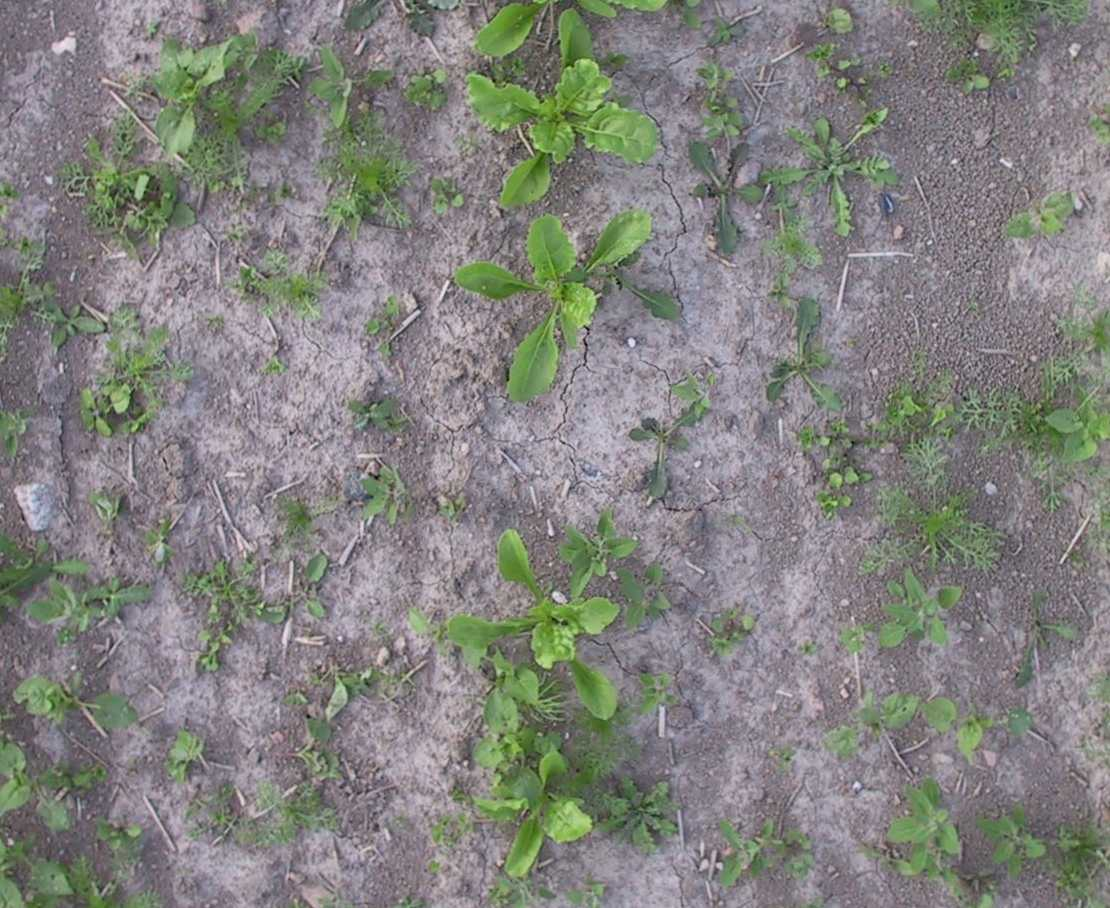
\includegraphics[width=6cm]{img/image.jpg}
\caption{Et billede af nogle sukkerroer.}
\label{figEtBilledeAfNogleSukkerroer}
\end{figure}

Vi kan også skrive noget matematik, eksempelvis 
Pythagoras' læresætning
\begin{align}
a^2 + b^2 = c^2
\end{align}

\section{Konklusion}

Latex virker \ldots


\printbibliography
\end{document}
